\documentclass{article}

\usepackage{graphicx}
\usepackage{imakeidx}
\usepackage{url}
\usepackage{listings}
\usepackage{color}

\definecolor{bluee}{rgb}{0,1,0}

\begin{document}

\clearpage
\thispagestyle{empty}

\begin{center}
\Large\textbf{Assignment - 8}
\vspace*{1\baselineskip}
\\
\LARGE\textbf{ELP - 780 Software Lab}
\vspace*{1\baselineskip}
\\
\Large\textbf{Prateek Arora}
\\
\Large\textbf{2017EET2841}
\\
\Large\textbf{2017-19}
\\
\vspace*{1\baselineskip}
Python and Github
\\
\vspace*{5\baselineskip}

\includegraphics[scale = 0.8]{logo} %%height=width =
\\
\vspace*{2\baselineskip}
Computer technology
\\IIT Delhi
\\India
\vspace*{1\baselineskip}
\\Sept 27, 2018
\end{center}

\tableofcontents
\setcounter{page}{1}
\newpage


\section{Problem Statement-1}
\subsection{Problem Statement}
\begin{itemize}
\item Find the two largest valid crosses that can be drawn on smart cells in the grid, and return two integers denoting the dimension of the each of the two largest valid crosses.
\item The two crosses cannot overlap, and the dimensions of each of the valid crosses should be maximal.
\end{itemize}
\subsection{Assumptions}
\begin{itemize}
\item 2 $\leq$ n $\leq$ 105
\item 2 $\leq$ m $\leq$ 105
  \end{itemize}
\subsection{Program Structure}
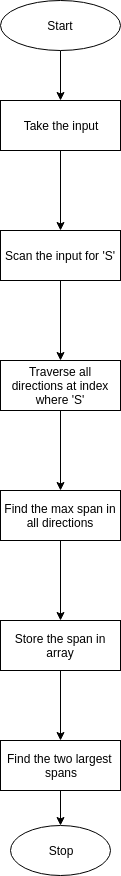
\includegraphics[scale=0.4]{ps1c}
\subsection{Algorithm and Implementation}
\begin{enumerate}
\item Take the input
\item Scan the input for 'S'.
\item Traverse all directions at index where 'S'.
\item Find the max span in all directions.
\item Store the span in array
\item Find the two largest spans  
\end{enumerate}
\subsection{Input and Output format}

\textbf{Input Format} 
\begin{itemize}
\item "row" "col"
\item "string matrix"
\end{itemize}

\noindent \textbf{Output Format} 
\begin{itemize}
\item "max1" "max2"
\end{itemize}

\subsection{Difficulties/Issues Faced}
\begin{itemize}
\item Finding nonoverlapping crosses.  
\end{itemize}

\subsection{Screenshots}
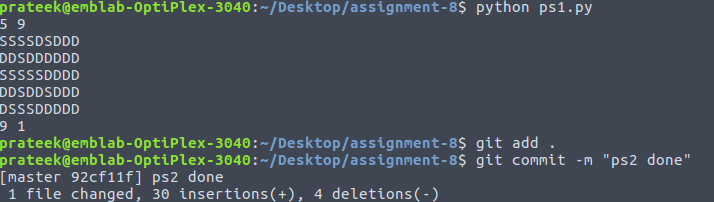
\includegraphics[scale = 0.5]{ps1}\\ \\

\section{Problem Statement-2}
\subsection{Problem Statement}
After, getting mix results of valid crosses, professors decided to test the computation abilities on one more problem. This time professors wanted to test the decryption capabilities of the computer. \\
Encryption of  a message requires three keys, k1, k2, and k3. The 26 letters of English and underscore are divided in three groups \\
Within each group the letters are rotated left by ki positions in the message. Each group is rotated independently of the other two. Decrypting the message means doing a right rotation by ki positions within each group.
\subsection{Assumptions}
\begin{itemize}
\item 1 $\leq$ Length of the string $\leq$ 150
\item 1 $\leq$ ki $\leq$ 150 (i=1,2,3)
\end{itemize}
\subsection{Program Structure}
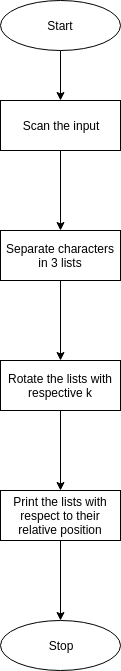
\includegraphics[scale = 0.5]{ps2c}
\subsection{Algorithm and Implementation}
\begin{enumerate}
\item Scan the input.
\item Separate characters in 3 lists.
\item Rotate the lists with respective k
\item Print the lists with respect to their relative position.  
\end{enumerate}
\subsection{Input and Output format}
\textbf{Input} \\
k1 k2 k3 \\
"encrypted string" \\
\textbf{Output} \\
"decrypted string"
\subsection{Difficulties/Issues Faced}
\begin{itemize}
\item Rotating the list.\cite{grep}
\end{itemize}

\subsection{Screenshots}
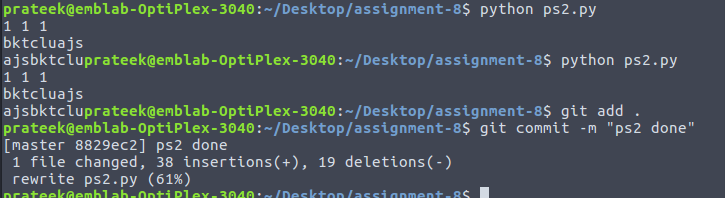
\includegraphics[scale = 0.5]{ps2}\\ \\

\pagebreak
\section{Appendix}
\subsection{Appendix A: Code for ps1}

\lstset{
numbers = left,
commentstyle=\color{bluee}}

\begin{lstlisting}[language=Python]
# scan row and col
row, col = input().split()
# scan the input
s = []
for i in range(int(row)):
    str = input()
    s.append(str)
# var to store various counts
count = 0
num = 1
flag = 0

maxlist = []
# scan the string and check for valid plus
for i in range(int(row)):
    for j in range(int(col)):
        flag = 0
        if s[i][j] == 'S':
            flag = 1
            num = 1
            count = 0
            while i - num >= 0 and i + num < int(row) and j - num >= 0 and j + num < int(col) and s[i-num][j] == 'S' and s[i][j-num] == 'S' and s[i+num][j] == 'S' and s[i][j+num] == 'S':
                    count += 1
                    num += 1
        if flag == 1:
            maxlist.append(count*4 + 1)
# max1 and max2 for 2 largest
max1 = 0
max2 = 0
# find two largest

if (len(maxlist) == 0):
    print("0, 0")
else:
    for i in range(len(maxlist)):
        if maxlist[i] >= max1:
            max2 = max1
            max1 = maxlist[i]
    print (max1, max2)


\end{lstlisting}
\subsection{Appendix B: Code for ps2}

\begin{lstlisting}[language=Python]

# for all 3 rotations
k1, k2, k3 = input().split()
str = input()
# separating the characters
first = []
second = []
third = []
for i in str:
    if ord(i) >= ord('a') and ord(i) <= ord('i'):
         first.append(i)
    elif ord(i) >= ord('j') and ord(i) <= ord('r'):
         second.append(i)
    else:
         third.append(i)

#Roatating the lists

first_r = (first[-int(k1):] + first[:-int(k1)])
second_r = (second[-int(k2):] + second[:-int(k2)])
third_r = (third[-int(k3):] + third[:-int(k3)])

ctr1 = 0
ctr2 = 0
ctr3 = 0

#printing the result

for i in str:
    if ord(i) >= ord('a') and ord(i) <= ord('i'):
         print(first_r[ctr1],end = '')
         ctr1 += 1
    elif ord(i) >= ord('j') and ord(i) <= ord('r'):
         print(second_r[ctr2],end = '')
         ctr2 += 1
    else:
         print(third_r[ctr3],end = '')
         ctr3 += 1

\end{lstlisting}

\begin{thebibliography}{1}

\bibitem{grep}
  \color{blue}\url{https://stackoverflow.com/questions/9457832/python-list-rotation}

\end{thebibliography}

\end{document}